% !TeX spellcheck = en_GB
% !TeX program = pdflatex
%
% LuxSleek-CV 1.1 LaTeX template
% Author: Andreï V. Kostyrka, University of Luxembourg
%
% 1.1: added tracking and letter-spacing for prettier lower caps, added `~` for language levels
% 1.0: initial release
%
% This template fills the gap in the available variety of templates
% by proposing something that is not a custom class, not using any
% hard-coded settings deeply hidden in style files, and provides
% a handful of custom command definitions that are as transparent as it gets.
% Developed at the University of Luxembourg.
%
% *NOTHING IS HARCODED, and never should be.*
%
% Target audience: applicants in the IT industry, or business in general
%
% The main strength of this template is, it explicitly showcases how
% to break the flow of text to achieve the most flexible right alignment
% of dates for multiple configurations.

\documentclass[11pt, a4paper]{article} 

\usepackage[T1]{fontenc}     % We are using pdfLaTeX,
\usepackage[utf8]{inputenc}  % hence this preparation
\usepackage[british]{babel}  
\usepackage[left = 0mm, right = 0mm, top = 0mm, bottom = 0mm]{geometry}
\usepackage[stretch = 25, shrink = 25, tracking=true, letterspace=30]{microtype}  
\usepackage{graphicx}        % To insert pictures
\usepackage{xcolor}          % To add colour to the document
\usepackage{fontawesome5}        % Provides icons for the contact details

\usepackage{enumitem}        % To redefine spacing in lists
\setlist{parsep = 0pt, topsep = 0pt, partopsep = 1pt, itemsep = 1pt, leftmargin = 6mm}

\usepackage[hidelinks]{hyperref}


\usepackage{FiraSans}        % Change this to use any font, but keep it simple
\renewcommand{\familydefault}{\sfdefault}

\definecolor{cvblue}{HTML}{304263}

%%%%%%% USER COMMAND DEFINITIONS %%%%%%%%%%%%%%%%%%%%%%%%%%%
% These are the real workhorses of this template
\newcommand{\dates}[1]{\hfill\mbox{\textbf{#1}}} % Bold stuff that doesn’t got broken into lines
\newcommand{\is}{\par\vskip.5ex plus .4ex} % Item spacing
\newcommand{\smaller}[1]{{\small$\diamond$\ #1}}
\newcommand{\headleft}[1]{\vspace*{3ex}\textsc{\textbf{#1}}\par%
    \vspace*{-1.5ex}\hrulefill\par\vspace*{0.7ex}}
\newcommand{\headright}[1]{\vspace*{2.5ex}\textsc{\Large\color{cvblue}#1}\par%
     \vspace*{-2ex}{\color{cvblue}\hrulefill}\par}
%%%%%%%%%%%%%%%%%%%%%%%%%%%%%%%%%%%%%%%%%%%%%%%%%%%%%%%%%%%%

\begin{document}

% Style definitions -- killing the unnecessary space and adding the skips explicitly
\setlength{\topskip}{0pt}
\setlength{\parindent}{0pt}
\setlength{\parskip}{0pt}
\setlength{\fboxsep}{0pt}
\pagestyle{empty}
\raggedbottom

\begin{minipage}[t]{0.33\textwidth} %% Left column -- outer definition
%  Left column -- top dark rectangle
\colorbox{cvblue}{\begin{minipage}[t][5mm][t]{\textwidth}\null\hfill\null\end{minipage}}

\vspace{-.2ex} % Eliminates the small gap
\colorbox{cvblue!90}{\color{white}  %% LEFT BOX
\kern0.09\textwidth\relax% Left margin provided explicitly
\begin{minipage}[t][293mm][t]{0.82\textwidth}
\raggedright
\vspace*{2.5ex}

\Large Riccardo \textbf{\textsc{Maldini}} \normalsize 

% Centering without extra vertical spacing
\null\hfill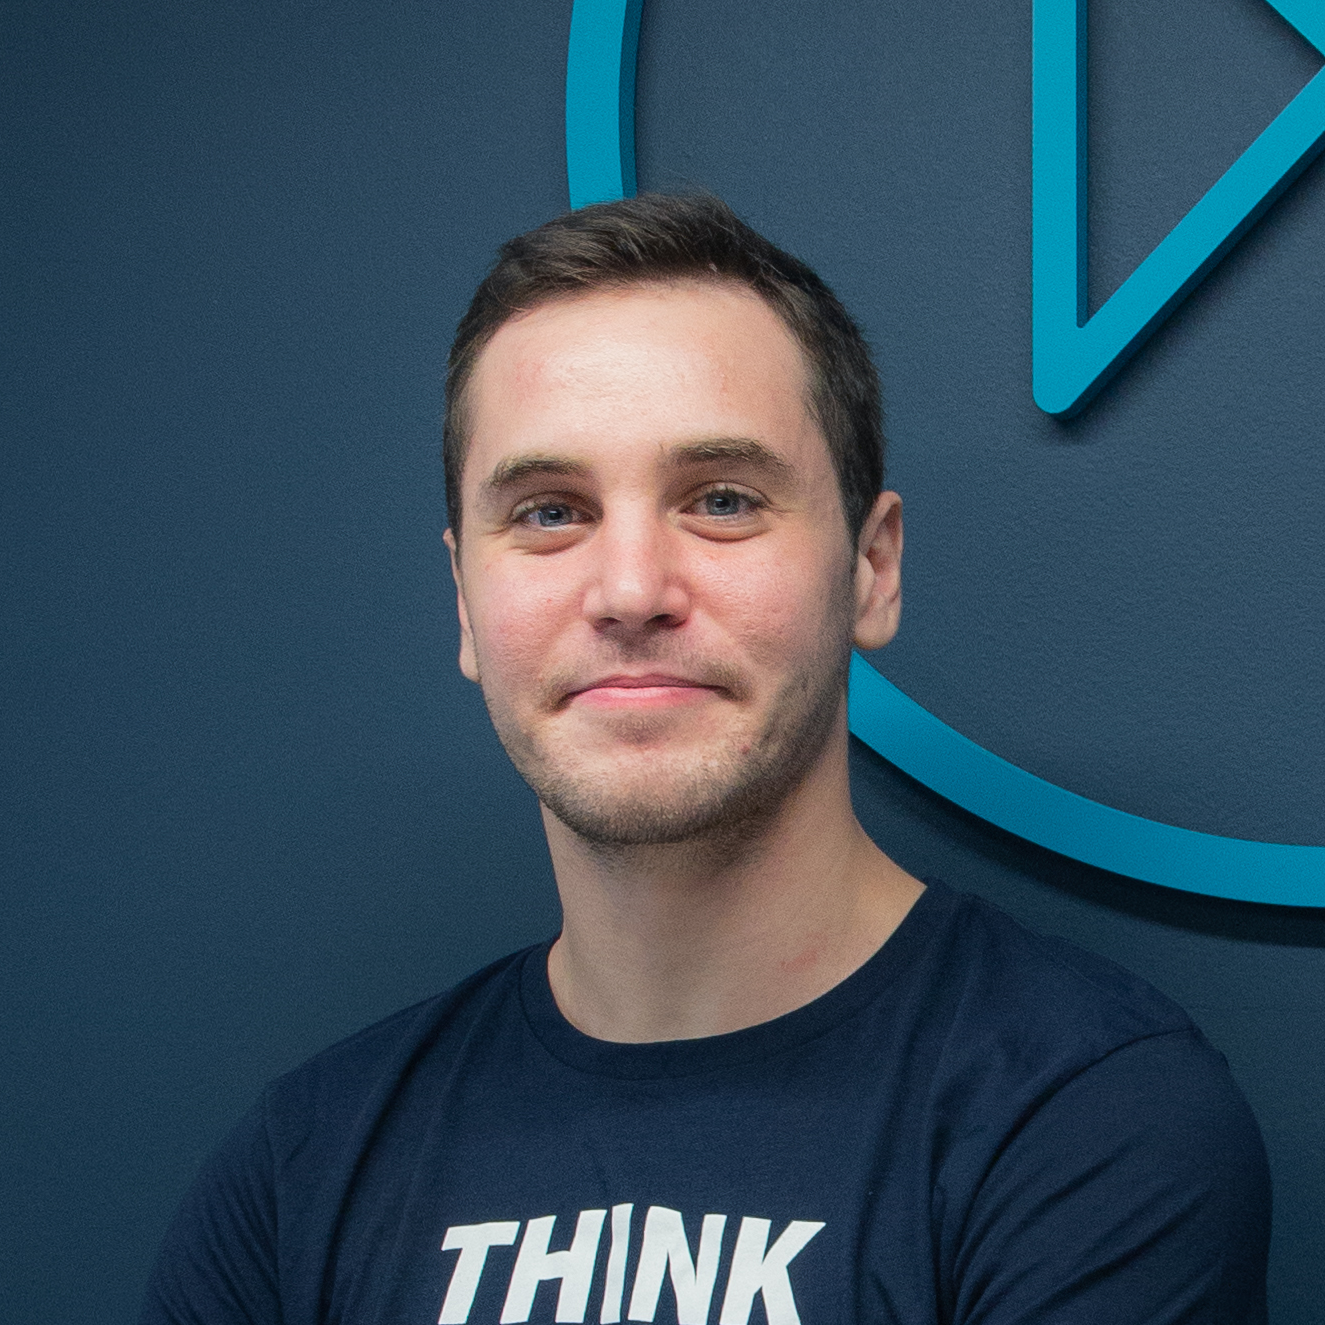
\includegraphics[width=0.50\textwidth]{profile.png}\hfill\null

\vspace*{0.5ex} % Extra space after the picture

\headleft{Profile Summary}
\small
\textit{Backend Software Engineer} with over 3 years of experience in software design and development, specializing in Java Spring Boot. MSc in Software Engineering.

\headleft{Contact information}
\faHome\ \ Milano\\[0.5ex]
\faEnvelope\ \ \href{mailto:riccardo.maldini@gmail.com}{riccardo.maldini@gmail.com} \\[0.5ex]
\faPhone\ \ \href{tel:393317767246}{+39\,331\,776\,7246}
 \\[0.5ex]
\faGlobeAmericas\ \ \href{https://www.riccardomaldini.it}{riccardomaldini.it}\\[0.5ex]
\faGithub\ \  \href{https://github.com/maldins46}{maldins46}

\headleft{Languages}
\textbf{Italian} Native speaker \\[0.5ex]
\textbf{English} Professional proficiency \\[0.5ex]

\headleft{Skills and expertise}
\textbf{Engineering foundations} 
Proficient in applying SOLID principles and software design patterns to create scalable and maintainable systems. Experienced with Agile methodologies, CI/CD automation (GitLab Pipelines), and build automation tools (Gradle, Maven). Strong team organizational skills, honed through practical application of Agile frameworks.\\[0.5ex]

\textbf{Backend Development} Proficiency in Java, with a focus on the Spring Boot framework. Expertise in developing RESTful APIs and implementing the MVC pattern. Worked with relational (MySQL, SQLite) and non-relational (MongoDB) databases.\\[0.5ex]

\textbf{Web \& Mobile Development} Hands-on experience with the MEAN stack through academic and personal projects. Proficient in Java for Android native development using Jetpack and skilled in experimenting with Flutter for academic projects.


\end{minipage}%
\kern0.09\textwidth\relax%%Right margin provided explicitly to stretch the colourbox
}
\end{minipage}% Right column
\hskip2.5em% Left margin for the white area
\begin{minipage}[t]{0.56\textwidth}
\setlength{\parskip}{0.8ex}% Adds spaces between paragraphs; use \\ to add new lines without this space. Shrink this amount to fit more data vertically

\vspace{2ex}

\headright{Work Experience}

\textsc{Software Engineer}
\dates{June 2022 - Now}\\
at \textit{MDOTM Srl}, Milano (MI)  

\smaller{Maintainer and reviewer of the External Backend Layer of the system. Supported (and lately, led)  architectural design and development efforts in this functional area.}

\smaller{Developed new features in an Agile Scrum framework with an API-first approach. Enhanced onboarding by introducing structured documentation, both auto-generated (Maven Site) and manual (SDD).}

\smaller{Stack: Spring Boot, MongoDB, MySQL, ActiveMQ. Technologies: JUnit, Mockito, gRPC, AWS, Sonar, ELK, Grafana, Draw.io, GitLab Pipelines.}\is

\textsc{Jr. Software Developer}
\dates{August 2021 - June 2022}\\ 
at \textit{MDOTM Srl}, Milano (MI)  

\smaller{Developed algorithms for financial market analysis to support the Financial Research Team.}

\smaller{Facilitated the transition of the Backend Core Layer from a legacy system to a modular, testable architecture. Advocated for and implemented unit testing practices using JUnit and Mockito.}

\smaller{Stack: Spring Boot, MySQL, ActiveMQ. Technologies: JUnit, Mockito, Flask, Python Notebooks, GitLab Pipelines.}\is


\textsc{Web Game Designer}
\dates{April 2019 - June 2019}\\
at \textit{Digit Srl}, Urbino (PU)  

\smaller{Full-stack development of a \href{https://codycolor.codemooc.net}{\textit{multiplayer online game}}, devised to teach computational thinking to young learners.}

\smaller{Managed online lobbies hosting hundreds of simultaneous players.}

\smaller{Stack: MEAN (MongoDB, Express, Angular, Node.js). Technologies: RabbitMQ, Firebase Auth, STOMP, WebSockets.}

\headright{Education}

\textsc{MSc in “Ingegneria e Scienze Informatiche”}\dates{2019 - 2021}\\
at \textit{Alma Mater Studiorum - Università di Bologna}\\[0.4ex]
\smaller{Closed with full marks with honors (110/110 e Lode)}\is


\textsc{BSc in “Informatica Applicata”}\dates{2016 - 2018}\\
at \textit{Università degli Studi di Urbino Carlo Bo} \\[0.4ex]
\smaller{Closed with full marks with honors (110/110 e Lode)} 



\headright{Projects}

\smaller{\textbf{\href{https://maldins46.github.io/CovidAnalysis}{CovidAnalysis}} An open-source project featuring a Python module and Angular client for extracting and visualizing semi-real-time COVID-19 open data.} 

\smaller{\textbf{\href{https://play.google.com/store/apps/details?id=com.maldini.riccardo.betassist&hl=it&pli=1}{BetAssist}} An Android app providing betting tips, forecasts, bet slip organization, and live scores. The app uses a native Java frontend and a mixed backend approach (Heroku cron jobs + Cloud Firestore) to process live data from an open football data API.}

\smaller{\textbf{\href{https://www.researchgate.net/publication/336734066_CodyColor_Design_of_a_Massively_Multiplayer_Online_Game_to_Develop_Computational_Thinking_Skills}{CodyColor} \& \href{https://www.researchgate.net/publication/340683343_Digital_Ariadne_Citizen_Empowerment_for_Epidemic_Control}{Digital Ariadne}} Co-authored academic publications as part of initial work experience, contributing to projects designed to enhance computational learning.}

\smaller{More contributions and details are available at \textbf{\href{https://www.riccardomaldini.it}{riccardomaldini.it}}}

\end{minipage}

\end{document}
